% !TeX root = ../main.tex
\documentclass[./../main.tex]{subfiles}

\begin{document}

Bài kiểm thử sẽ được đánh giá thành hai bài thử nghiệm
\begin{enumerate}
	\item Bài thử nghiệm tự phát triển được em tự triển khai với mục đích đánh
	      giá các chức năng được phát triển có thể xác minh và khai các lỗ hổng
	      đã được phát triển hay không.
	\item Bài thử nghiệm thực tế thứ hai đánh giá trên một tập môi trường là dự án các dự án Vulnerables Web Application phát triển cho thử nghiệm các lỗ hổng ứng dụng.
\end{enumerate}

\section{Bài thử nghiệm tự phát triển}

Để đánh giá được lỗ hổng, em tự xây dựng một bài kiểm tra cho công cụ kiểm thử tự động ở trên. Để tập trung vào lỗ hổng đã xây dựng, em chỉ xây dựng các lỗ hổng cho công cụ mình có thể khai thác. Các lỗ hổng khác sẽ nằm ngoài phạm vi đánh giá của bài thử nghiệm này.

\subsection{Môi trường thử nghiệm}

\begin{description}
	\item[Ngôn ngữ] PHP 7.2 và Python.
	\item [Cơ sở dữ liệu] MySql 5.7.38
	\item [Môi trường triển khai] Docker.
\end{description}

\subsection{Các chức năng và lỗ hổng}

Việc xây dựng một ứng dụng hoàn chỉnh để thử nghiệm sẽ rất khó,
do đó em xây dựng ứng dụng gồm các phần bị lỗi. Mỗi phần sẽ có một lỗi riêng
theo từng chức năng.

\subsubsection{Tìm kiếm người dùng}

\begin{description}
	\item[Mô tả] Chức năng cho phép tìm kiếm người dùng khi nhập đúng
	      thông tin gồm username và password \ref{src:sqli}.
	\item [Loại lỗ hổng] SQL Injection.
\end{description}

\subsubsection{Xem thông tin tên miền}

\begin{description}
	\item[Mô tả] Chức năng cho sử dụng câu lệnh `host` của hệ thống để đưa ra thông tin về ip, tên miền của website được nhập vào \ref{src:cmdi}.
	\item[Loại lỗ hổng] Command Injection.
\end{description}

\subsubsection{Biểu diễn trang}

\begin{description}
	\item[Mô tả] trang để biểu diễn một đoạn từ file khác được bằng cách
	      include file vào nhưng cho phép người dùng điều chính tên trang \ref{src:rfi}.
	\item[Loại lỗ hổng] Path Traversal, Local File Inclusion, Remote
	      File Inclusion.
\end{description}

\subsubsection{Xin chào}

\begin{description}
	\item[Mô tả] Một trang cho phép nhập tên người dùng để in ra sử dụng một template engine \ref{src:ssti}.
	\item[Loại lỗ hổng] Server Side Template Injection.
\end{description}


\subsection{Kết quả trên môi trường thử nghiệm}

Kết quả việc tự động kiểm thử và sử dụng tính năng tự xác minh lỗi
hổng được phát triển \ref{fig:result_test} và \ref{tb:result_test}.

\begin{figure}[h!]
	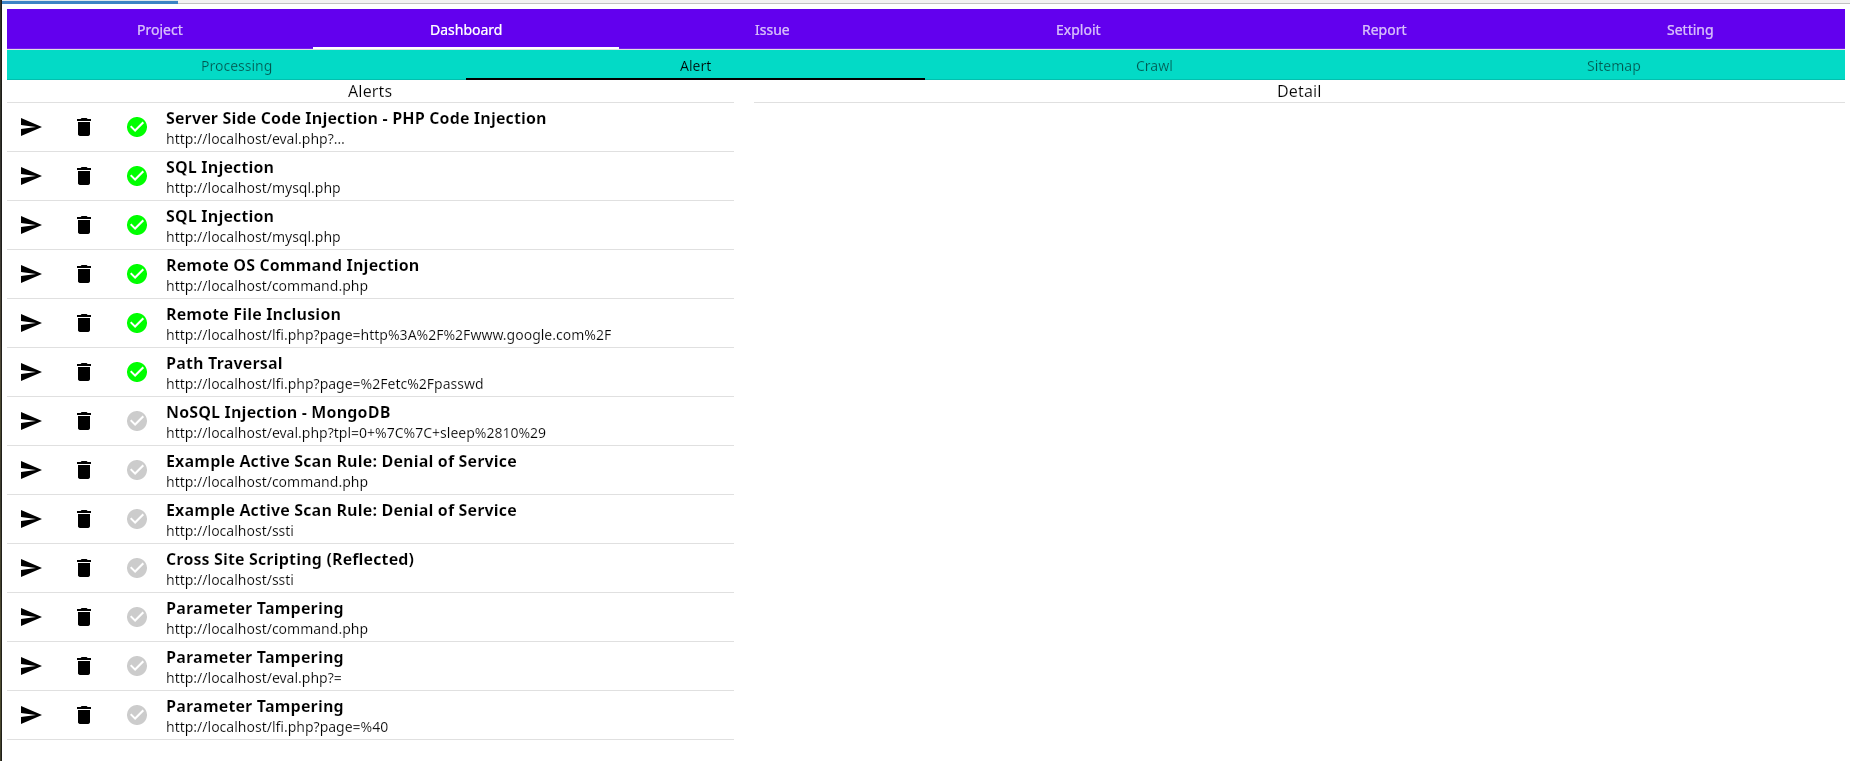
\includegraphics[width=\linewidth]{./images/naf_result.png}
	\caption{Kết quả đánh thử nghiệm của NAF trên môi trường tự phát triển}
	\label{fig:result_test}
\end{figure}

Đồng thời đánh giá với Invicti (Nesparker) 5.8.1 là một công cụ thương mại, em được kết quả như sau \ref{fig:np_vulns}.

\begin{figure}[h!]
	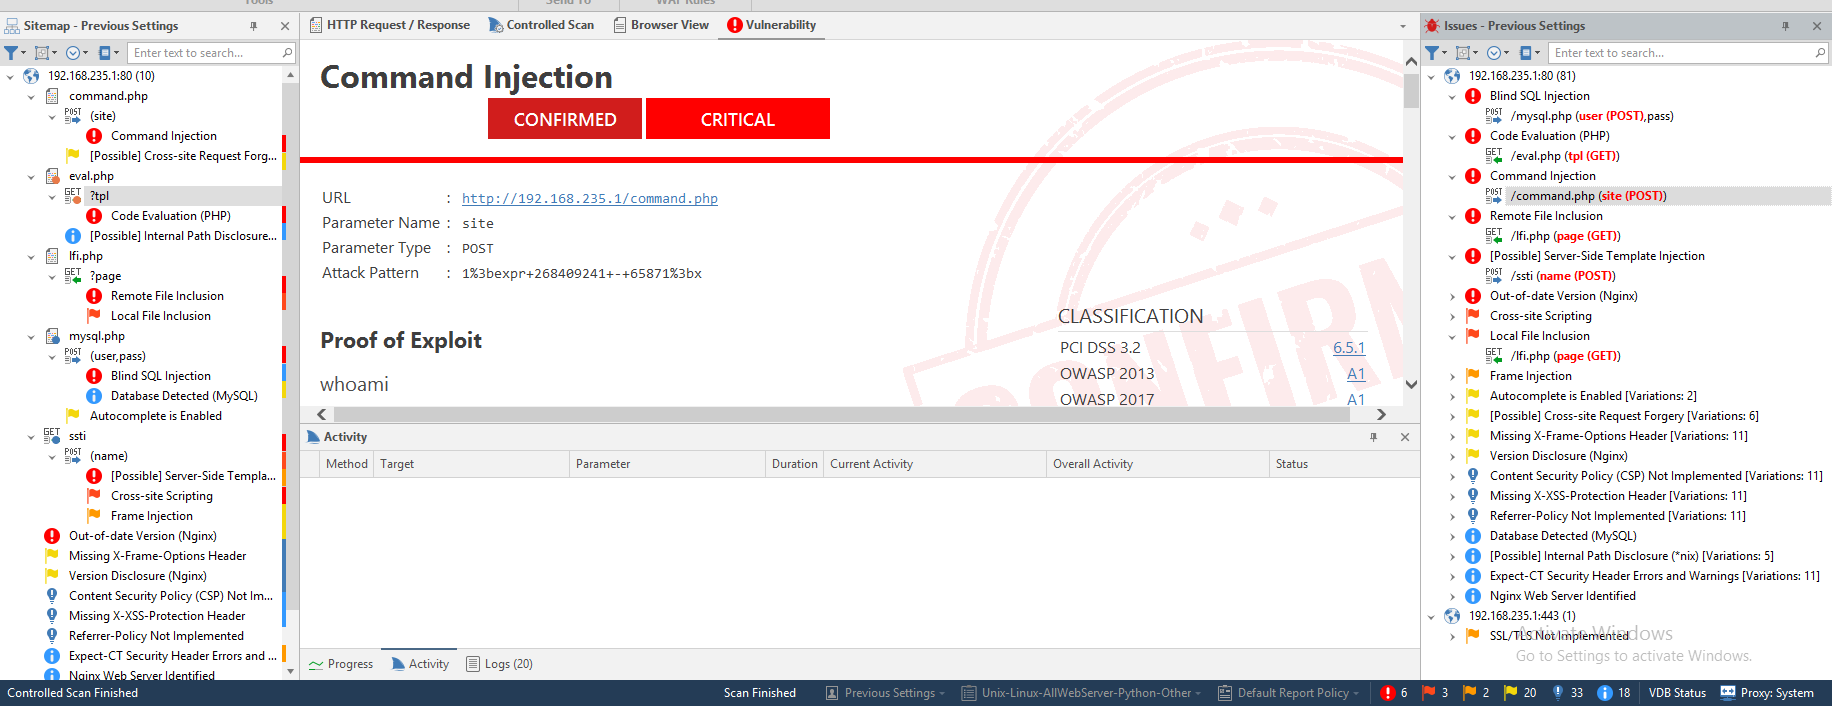
\includegraphics[width=\linewidth]{./images/np.png}
	\caption{Kết quả đánh thử nghiệm của Invicti trên môi trường tự phát triển}
	\label{fig:np_vulns}
\end{figure}


\begin{table}[ht!]
	\begin{tabular}{|l|ll|ll|}
		\hline
		\multirow{2}{*}{\textbf{Lỗ hổng}} & \multicolumn{2}{l|}{\textbf{Đã xác minh}} & \multicolumn{2}{l|}{\textbf{Khai thác}}                                      \\ \cline{2-5}
		                                  & \multicolumn{1}{l|}{NAF}                  & Invicti                                 & \multicolumn{1}{l|}{NAF} & Invicti \\ \hline
		Server Side Template Injection    & \multicolumn{1}{l|}{Không}                & Có                                      & \multicolumn{1}{l|}{Có}  & Không   \\ \hline
		Evaluation Code                   & \multicolumn{1}{l|}{Có}                   & Có                                      & \multicolumn{1}{l|}{Có}  & Có      \\ \hline
		OS Command Injection              & \multicolumn{1}{l|}{Có}                   & Có                                      & \multicolumn{1}{l|}{Có}  & Có      \\ \hline
		SQL Injection                     & \multicolumn{1}{l|}{Có}                   & Có                                      & \multicolumn{1}{l|}{Có}  & Có      \\ \hline
		Remote File Inclusion             & \multicolumn{1}{l|}{Có}                   & Có                                      & \multicolumn{1}{l|}{Có}  & Có      \\ \hline
		Local File Inclusion              & \multicolumn{1}{l|}{Có}                   & Có                                      & \multicolumn{1}{l|}{Có}  & Có      \\ \hline
	\end{tabular}
	\caption{Kết quả việc thử nghiệm trên môi trường tự phát triển}
	\label{tb:result_test}
\end{table}

Nhận xét: Số lượng lỗ hổng rà quét được của NAF khi sử dụng ZAP không đầy đủ so với Invicti do phụ thuộc vào các luật của cộng đồng phát triển, nhưng NAF đã khai thác tốt hơn với lỗ hổng Server Side Template Injection.


\section{Thử nghiệm trên dự án VWA}

Để phục vụ cho việc thử nghiệm kiểm thử hoặc mục đích học tập, một số đự án là các ứng dụng Web có chứa lỗ hổng được gọi là Vulnerables Web Application. Các dự án này thường có các lỗ hổng tương đối sát với thực tế nên em sẽ sử dụng các dự án này làm tập đầu vào cho việc thử nghiệm này.

\subsection{Về môi trường thử nghiệm}

Bài thử nghiệm sẽ gồm các bài kiểm thử sau
\begin{enumerate}
	\item DVWA \footnote{\url{https://dvwa.co.uk/}}
	\item Acunetix Acuart \footnote{\url{http://testaspnet.vulnweb.com/}}
	\item Acunetix Acublog \footnote{\url{http://testphp.vulnweb.com/}}
	\item Testsparker PHP \footnote{\url{http://php.testsparker.com/}}
\end{enumerate}

\subsection{Kết quả VWA}

Đầu tiên là kết quả về việc xác minh của NAF đánh giá lại đối với các trình rà quét của ZAP.

\begin{table}[ht!]
	\begin{tabular}{|l|r|r|r|}
		\hline
		\textbf{Lỗ hổng}      & \multicolumn{1}{l|}{\textbf{Rà quét tự động}} & \multicolumn{1}{l|}{\textbf{Xác thực}} & \multicolumn{1}{l|}{\textbf{Dương tính giả}} \\ \hline
		SQL Injection         & 15                                            & 13                                     & 2                                            \\ \hline
		OS Command Injection  & 2                                             & 2                                      & 0                                            \\ \hline
		Remote File Inclusion & 2                                             & 2                                      & 0                                            \\ \hline
		Local File Inclusion  & 2                                             & 2                                      & 0                                            \\ \hline
		Evaluation Code       & 1                                             & 1                                      & 0                                            \\ \hline
	\end{tabular}
	\caption{Kết quả xác minh của NAF}
\end{table}

Tiếp tục so sánh với Invicti(NetSparker), do vấn đề bản quyền nên bài kiểm thử `Testsparker PHP' sẽ không được thực hiện trên Invicti. Em thu được kết quả như \ref{tb:diff}. \textit{Lưu ý rằng bài thử nghiệm được bỏ qua chỉ ảnh hưởng đến lỗ hổng `OS Command Injection'.}

\begin{table}[ht!]
	\begin{tabular}{|l|r|r|}
		\hline
		\textbf{Lỗ hổng}      & \multicolumn{1}{l|}{\textbf{NAF}} & \multicolumn{1}{l|}{\textbf{Invicity}} \\ \hline
		SQL Injection         & 13                                & 18                                     \\ \hline
		OS Command Injection  & 1                                 & 1                                      \\ \hline
		Remote File Inclusion & 2                                 & 2                                      \\ \hline
		Local File Inclusion  & 2                                 & 2                                      \\ \hline
		Evaluation Code       & 1                                 & 1                                      \\ \hline
	\end{tabular}
	\caption{So sánh kết quả của quá trình rà quét tự động với Invicti}
	\label{tb:diff}
\end{table}

Nhận xét: Do số lượng cảnh báo được đưa ra ở phần rà quét đã thấp hơn nên dẫn đến kết quả của cuối cùng thấp hơn. Ngoài ra, các trình thu thập thông tin hoạt động kém hiệu quả cũng dần đến số lượng lỗ hổng phát hiện ra thấp hơn. Việc lượng lỗ hổng cảnh báo đưa ra có thể được cải thiện bằng cách cải thiện hoặc viết lại các luật sử dụng trong ZAP, nhưng nên chú ý rằng việc này có thể sẽ đem NAF rời xa khỏi việc tận dụng lợi thế của dự án mã nguồn mở. Việc tăng khả năng rà quét, thu thập thông tin là rất khó do đã gắn liền với ZAP Core và ZAP Addon khác.

\end{document}

